\chapter{Trotter-Suzuki Decomposition}
Since the publication of the Trotter product formula~\cite{trotter1959product}, a great effort has been carried out by mathematicians, to study possible approximations of the exponential operator. In particular, Masuo Suzuki has studied on the higher-order approximation throughout his carrier, leading to major results in this subject~\cite{suzuki1985decomposition,suzuki1990fractal,Suzuki1992387, suzuki1994quantum,Suzuki1995425,suzuki1997algebraic,Suzuki200032}.

The Trotter product formula for the exponential of two not necessarily commuting linear operators reads as follows:
\begin{equation} \label{eq:trotter}
\exp{(A+B)} = \lim_{n\rightarrow\infty} \left(\exp\left({\frac{A}{n}}\right) \exp{\left(\frac{B}{n}\right)}\right)^n.
\end{equation}
The Trotter-Kato theorem defines the properties that the operators $A$ and $B$ must satisfy for the Eq.~\eqref{eq:trotter} to hold~\cite{KatoTosio1978}. In the simplest case, $A$ and $B$ can be seen as arbitrary $n\times n$ real or complex matrices, and the Eq.~\eqref{eq:trotter} reduces to the Lie product formula~\cite{SophusLie1888}. The exponential of a generic operator is usually difficult to calculate, but whenever this operator can be expressed as a sum of two operators $A$ and $B$, whose exponentiation is known, Eq.~\eqref{eq:trotter} provides a method to estimate $\exp{(A+B)}$. However, for practical purpose, this formula is not appropriate since it requires to take the limit for $n$ that goes to infinity. On a practical side, we could calculate the right side of the equation only for a finite value of $n$, leading to an approximation of the original problem. At this point, it becomes important to study what can be an efficient approximation of the exponential, and how to estimate the error.

%%%%%%%%%%%%%%%%%%%%%%%%%%%%%%%%%%%%%%%%%%%%%%%%%%%%%%%%%%%%%%%%%%%%%%%%%%%%%%%
\section{Exponential operator in physics}
First of all, let us discuss as to why we have to treat the exponential operator and why we need an approximant to treat it. The exponential operator appears in various fields of physics as a formal solution of the differential equation of the following form:
\begin{equation} \label{eq:general}
\dfrac{\partial}{\partial t} x(t) = M x(t),
\end{equation}
where $x$ is a function or a vector and $M$ is a finite or infinite dimensional operator. Typical examples include the Schr\"odinger equation
\begin{equation}
\imath\hbar\dfrac{\partial}{\partial t} \psi(t) = H\psi(t),
\end{equation}
the Hamiltonian equation
\begin{equation}
\dfrac{d}{d t} 
\begin{pmatrix}
\vec{p}(t) \\ \vec{q}(t)
\end{pmatrix}
= H
\begin{pmatrix}
\vec{p}(t) \\ \vec{q}(t)
\end{pmatrix},
\end{equation}
and the diffusion equation with a potential
\begin{equation}
\dfrac{d}{dt}P(x,t) = \emph{L} P(x,t).
\end{equation}
A formal solution of \eqref{eq:general} is given in the form of the Green's function as 
\begin{equation}
x(t) = G(t;0)x(0) = \exp\left({tM}\right)x(0).
\end{equation}
However, obtaining the Green's function $G(t;0) = \exp{(tM)}$ is as difficult as solving the equation \eqref{eq:general} in any other way. Another important instance of the exponential operator is the partition function in equilibrium quantum statistical physics:
\begin{equation}
Z = Tr\left(\exp\left({- \beta H}\right)\right).
\end{equation}

The exponential operator, however, is hard to compute in most interesting cases. The computation of the exponential operator $\exp{(xM)}$ becomes straightforward when a basis that diagonalize the operator $M$ is easy to obtain. In quantum many-body problems, however, the basis of the diagonalized representation is often nontrivial, because we are typically interested in the Hamiltonian with two terms or more that are mutually non-commutative; for example, the Ising model in a transverse field, written as follows:
\begin{equation} \label{eq:ising}
H = -\sum_{\langle i,j \rangle} J_{ij} \sigma_i^z \sigma_j^z - \triangle\sum_i \sigma_i^x
\end{equation}
and the Hubbard model,
\begin{equation} \label{eq:Hubbard}
H = -t \sum_{\sigma = \uparrow ,\downarrow} \sum_{\langle i,j \rangle} (c_{i\sigma}^\dagger c_{j\sigma} + c_{j\sigma}^\dagger c_{i\sigma}) + U\sum_i n_{i\uparrow} n_{i\downarrow}
\end{equation}
In the first example \eqref{eq:ising}, the quantization axis of the first term is the spin z axis, while that of the second term is the spin $x$ axis. The two terms are therefore mutually non-commutative. In the second example \eqref{eq:Hubbard}, the first term is diagonalizable in the momentum space, whereas the second term is diagonalizable in the coordinate space. In both examples, each term is easily diagonalizable. Since one quantization axis is different from the other, the diagonalization of the sum of the terms becomes difficult.

%%%%%%%%%%%%%%%%%%%%%%%%%%%%%%%%%%%%%%%%%%%%%%%%%%%%%%%%%%%%%%%%%%%%%%%%%%%%%%%
\section{Exponential product approximation}
As we have seen in the previous section, operator exponentiation plays a major role in most fields of physics. For this reason it is necessary to find good approximation to be able to calculate it. The Trotter-Suzuki approximation provides a way to deal with such operations. 

The simplest form of the Trotter-Suzuki approximation comes in the following form:
\begin{equation} \label{eq:approxexp}
\exp\left({x(A+B)}\right) = \exp\left({xA}\right)\exp\left({xB}\right) + O(x^2), 
\end{equation}
where $A$ and $B$ are arbitrary general operators with some commutation relation $[A,B] \neq 0$, and $x$ is a parameter. This equation is also known as the Trotter decomposition. To demonstrate that this is actually a first-order approximant, let us rearrange the formula in to following form:
\begin{equation}
\exp\left({xB}\right)\exp\left({xA}\right) = \exp\left({x(A+B) + O(x^2)}\right).
\end{equation}
We can calculate the form of the correction terms that appears in the exponent of the right-hand side by exploiting a Taylor expansion of both sides of the Eq.~\eqref{eq:approxexp}.
\begin{subequations} \label{eq:taylor-left}
\begin{align}
\exp\left({x(A+B)}\right) &= I + x(A+B) + \frac{1}{2} x^2 (A+B)^2 + O(x^3) \\
& = I + x(A+B) + \frac{1}{2} x^2 (A^2 + AB + BA + B^2) + O(x^3) 
\end{align}
\end{subequations}
for the left-hand side, and
\begin{subequations}  \label{eq:taylor-right}
\begin{align}
\exp\left({xA}\right)\exp\left({xB}\right) &= (I + xA + \frac{1}{2} x^2 A^2 + O(x^3)) (I + xB + \frac{1}{2} x^2 B^2 + O(x^3))\\
& = I + x(A+B) + \frac{1}{2} x^2 (A^2 + 2AB + B^2) + O(x^3)  
\end{align}
\end{subequations}
for the right-hand side. The two equations~\eqref{eq:taylor-left} and~\eqref{eq:taylor-right} differ as the operator $A$ always comes on the left of the operator $B$ in the latter, which let us write the form of the correction term:
\begin{equation}
\exp\left({xA}\right) \exp\left({xB}\right) = \exp\left({x(A+B) + \frac{1}{2} x^2 [A,B] + O(x^3)}\right)
\end{equation}
Therefore, dividing the parameter $x$ into $n$ slices, we get
\begin{align}
\left(\exp\left({\frac{x}{n}A}\right) \exp\left({\frac{x}{n}B}\right) \right)^n &= \left[ \exp\left({\frac{x}{n}(A + B) + \frac{1}{2}\left(\frac{x}{n}\right)^2 [A,B] + O\left(\left(\frac{x}{n}\right)^3\right)}\right) \right]^n \\
&= \exp\left({x(A+B) + \frac{1}{2}\left(\frac{x^2}{n}\right) [A,B] + O\left(\left(\frac{x^3}{n^2}\right)\right)}\right) 
\end{align}
and taking the limit $n \rightarrow \infty$ the correction term vanishes, recovering the exponential operator.

It is interesting to compare this approach with the one more frequently used perturbational approximation, namely
\begin{equation} \label{eq:roughapprox}
\exp\left({x(A+B)}\right) = I + x(A+B) + O(x^2).
\end{equation}
When dealing with Hermitian Hamiltonian $H=A+B$, the Trotter-Suzuki approximation has a remarkable advantage over the~\eqref{eq:roughapprox}. Indeed, in that scenario, the evolution operator is a unitary operator; the same is not true for the right-hand side of the Eq.~\eqref{eq:roughapprox}. Contrary, the Trotter-Suzuki preserves this property since it is a product of unitary operators. As a consequence, the norm of the wave function is preserved, resulting in a better accuracy of the evolution. However, a first-order approximation could not be enough  to achieve the high precision. For these reasons it is interesting to further develop the approximation, looking for higher order approximants.

%%%%%%%%%%%%%%%%%%%%%%%%%%%%%%%%%%%%%%%%%%%%%%%%%%%%%%%%%%%%%%%%%%%%%%%%%%%%%%%
\section{Fractal Decomposition}
To go beyond the simple approximation presented in the previous section, we can introduce a recursive approach, called Fractal Decomposition. Bearing in mind that we want to preserve the unitarity of the approximant, we are looking for an approximation of exponentials product.

The easiest improvement of the Trotter formula~\eqref{eq:approxexp} is the symmetrization
\begin{equation} 
S_2(x) \equiv \exp\left({\frac{x}{2}A}\right) \exp\left({xB}\right) \exp\left({\frac{x}{2}A}\right) = \exp\left({f(x)}\right).
\end{equation}
The symmetrized approximant has the property
\begin{equation}
S_2(-x) S_2(x) = \exp\left({-\frac{x}{2}A}\right) \exp\left({-xB}\right) \exp\left({-\frac{x}{2}A}\right) \exp\left({\frac{x}{2}A}\right) \exp\left({xB}\right) \exp\left({\frac{x}{2}A}\right) = I, \nonumber
\end{equation}
which prove that $f(x)$ does not have even-order term in $x$. Consequently, $S_2$ is a second-order approximant, with the following form
\begin{equation} \label{eq:S2-form}
S_2 = \exp\left({x(A+B) + x^3R_3 + x^5R_5 + \cdots}\right),
\end{equation}
where $R_i$ are suitable operators.

A fourth-order approximant can be constructed from the $S_2$ considering the product
\begin{subequations} \label{eq:fourth-order}
\begin{align} \label{eq:fourth-order.a}
S_4(x) = & S_2(sx) S_2((1-2s)x) S_2(sx) \\
= & \exp\left({\frac{s}{2}xA}\right) \exp\left({sxB}\right) \exp\left({\frac{1-s}{2}xA}\right) \exp\left({(1-2s)xB}\right) \cdot \nonumber \\
& \cdot \exp\left({\frac{1-s}{2}xA}\right) \exp\left({sxB}\right) \exp\left({\frac{s}{2}xA}\right),
\end{align}
\end{subequations}
where $s$ is an arbitrary real number. Using Eq.~\eqref{eq:S2-form} the expression~\eqref{eq:fourth-order} becomes
\begin{subequations} \label{eq:fourth-order2}
\begin{align} \label{eq:fourth-order2}
S(x) = & S_2(sx) S_2((1-2s)x) S_2(sx)	 \\
= & \exp\left({sx(A+B) + s^3x^3R_3 + O(x^5)}\right) \exp\left({(1-2s)x(A+B) + (1-2s)^3x^3R_3 + O(x^5)}\right) \nonumber \\
& \exp\left({sx(A+B) + s^3x^3R_3 + O(x^5)}\right) \\
= & \exp\left({x(A+B)+(2s^3+(1-2s)^3)R_3+O(x^5)}\right) \label{eq:fourth-order2.3}
\end{align}
\end{subequations}
The property $S(-x)S(x) = I$ also holds in this case, so we can conclude that the even-order correction in the exponent of~\eqref{eq:fourth-order2} will vanish, and the parameter $s$ must satisfy
\begin{equation} \label{eq:s}
2s^3 + (1-2s)^3 = 0.
\end{equation}
Solving Eq.~\eqref{eq:s}, we obtain $s = \frac{1}{2-\sqrt[3]{2}} = 1.351207$~. Suppose now that $S(x)$ is an approximation of the time-evolution operator, from time $t=0$ to $t=x$. The right term $S_2(sx)$ on the right-hand side of Eq.~\eqref{eq:fourth-order.a} evolves the system from $t=0$ to $t=sx>x$. The middle-term $S_2((1-2s)x)$ approximates the time evolution from $t=sx$ to $t=sx + (1-2s)x = (1-s)x$. Finally the last term $S_2(sx)$ approximates the evolution from $t=(1-s)x$ to $t=x$. Representing the evolution as in Fig.~\ref{plot:evolution}(a), it is evident that the evolution has a part that goes to the "past". In some cases this can be problematic, for instance when studying the diffusion from a delta peak as initial state. Indeed, in this case there is no past of the initial delta peak state. 

However, this problem can be easely solved by introducing another fourth-order approximant. Following the same idea, we consider
\begin{equation} \label{eq:fourth-order-nopast}
S_4(x) = S_2(s_2x)^2 S_2((1-4s_2)x) S_2(s_2x)^2	
\end{equation}
where $s_2$ is the parameter that solves the equation
\begin{equation}
4s_2^3 + (1-4s_2)^3 = 0, or s_2 = \frac{1}{4 - \sqrt[3]{4}}=0.414490\ldots
\end{equation}
Similarly to the $S(x)$ we represent $S_2(x)$ as in Fig.~\ref{plot:fractal-evolution}(b). Note that in this case the evolution remains between the initial and final time.
\begin{figure}
   \centering
   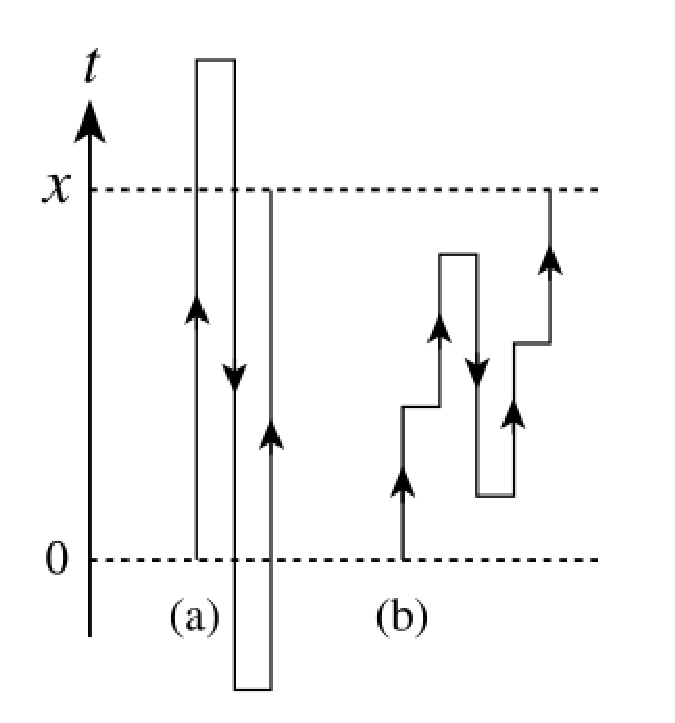
\includegraphics[width=5cm]{Plots/evolution.eps}
   \caption{Representation of the fourth-order approximation using (a) Eq.~\eqref{eq:fourth-order} and (b) Eq.~\eqref{eq:fourth-order-nopast}.} \label{plot:evolution}
\end{figure}


Now we can move to the sixth-order approximant, using $S_4(x)$ and following the same structure:
\begin{equation} \label{eq:sixth-order}
S_6(x) = S_4(s_4x)^2 S_4((1-4s_4)x) S_4(s_4x)^2,
\end{equation}
obtaining
\begin{equation}
4s_4^5 + (1-4s_4)^5 = 0,\quad \mathrm{or} \quad s_4 = \frac{1}{4-\sqrt[5]{4}} = 0.373065\ldots .
\end{equation}
We can continue this recursive procedure, ending up with the exact time evolution. It is interesting to note that this recursive procedure creates a fractal pattern composed by back-and-forth evolution, reproducing the exact time evolution.
\begin{figure}
  \centering
   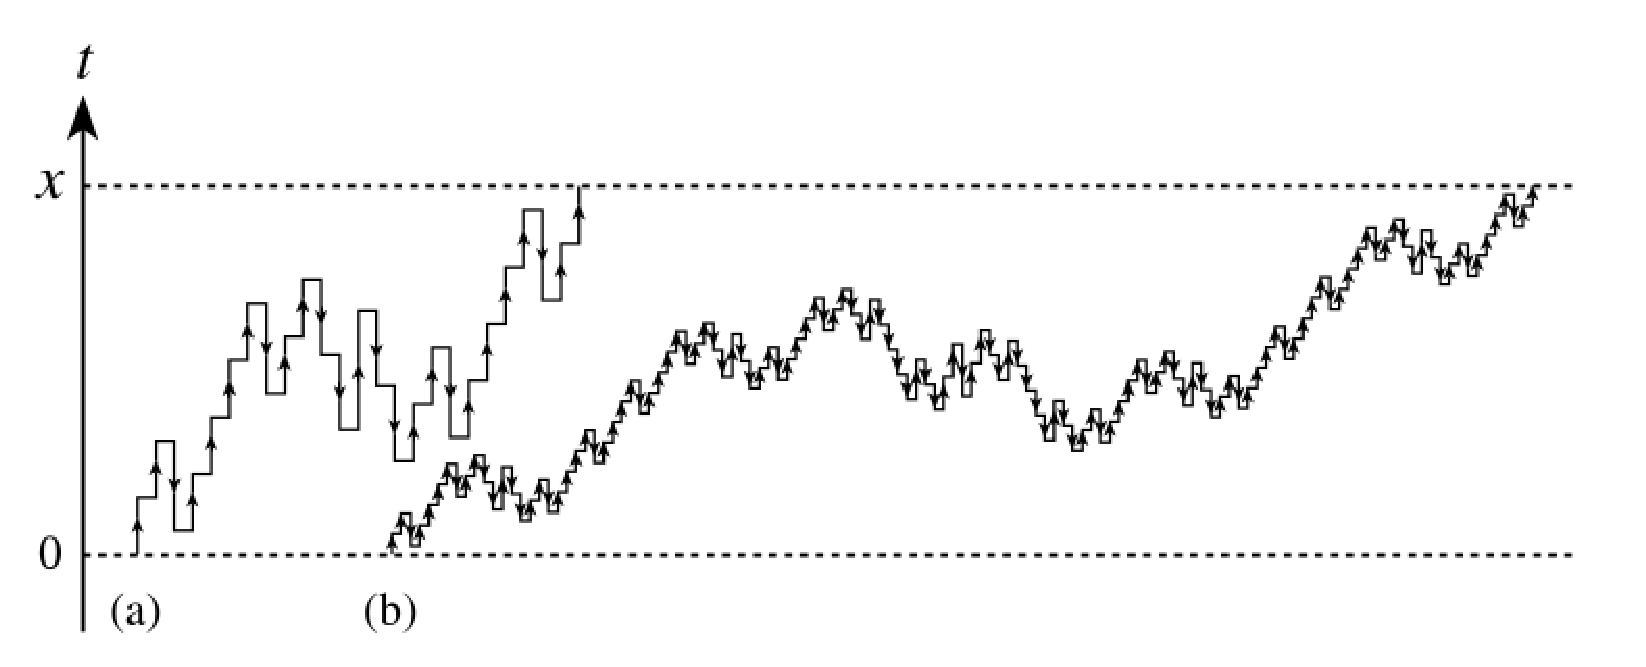
\includegraphics[width=8cm]{Plots/fractal_evolution.eps}
   \caption{Representation of the time evolution using (a) sixth-order approximant and (b) eighth-order approximant.} \label{plot:fractal-evolution}
\end{figure}

%%%%%%%%%%%%%%%%%%%%%%%%%%%%%%%%%%%%%%%%%%%%%%%%%%%%%%%%%%%%%%%%%%%%%%%%%%%%%%%
\section{Example: spin precession}
It is worth to give a brief and simple example to show some remarkable properties of the Trotter-Suzuki decomposition. In this section we compare it with the first order perturbation, using a simple example of quantum dynamics, namely the spin precession.

\begin{figure}[t]
  \centering
   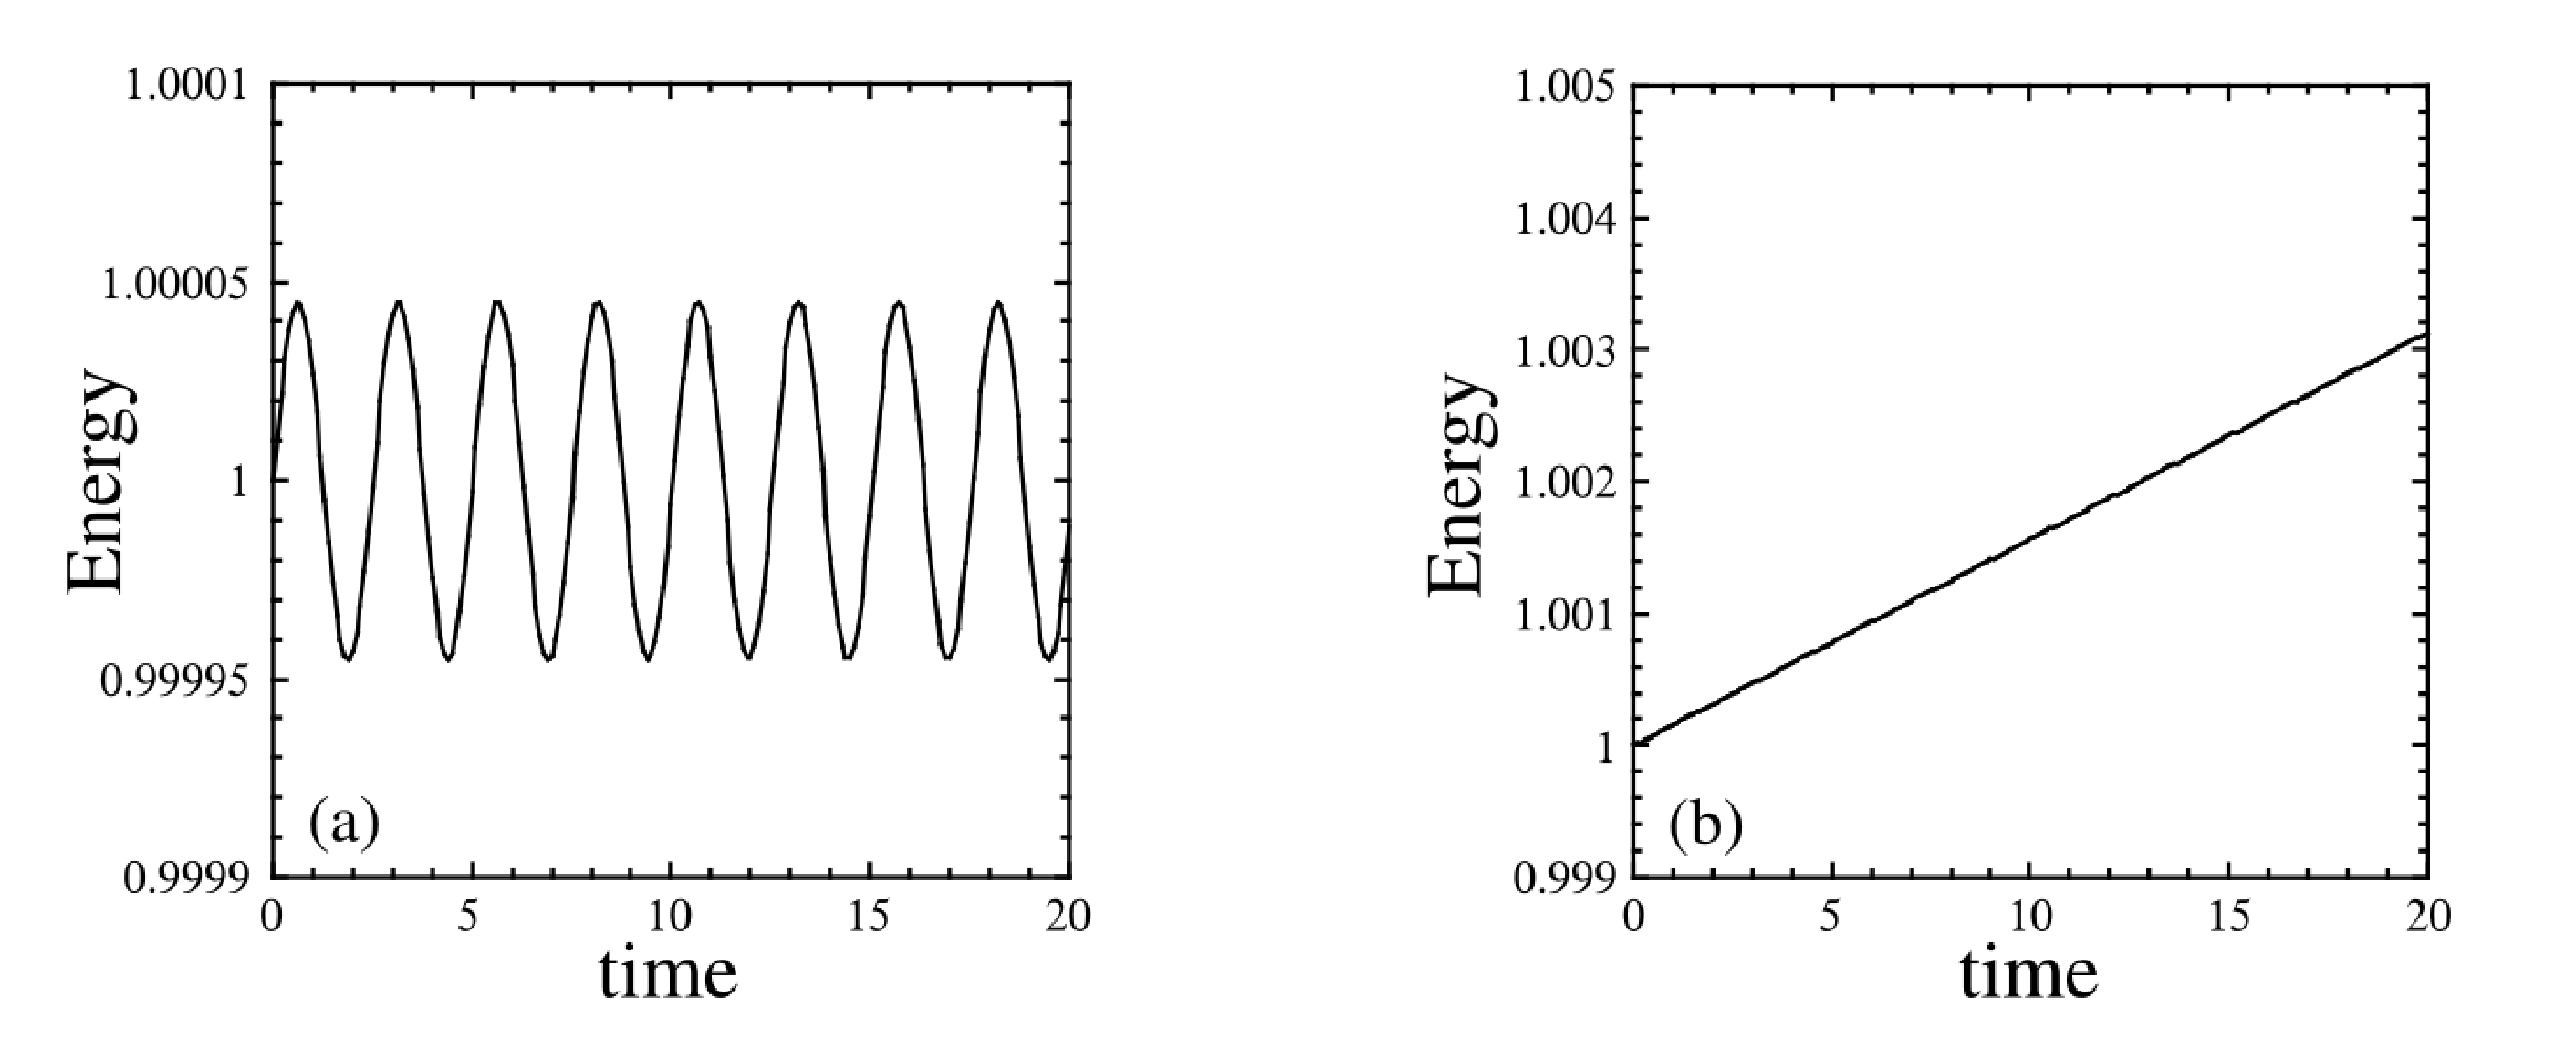
\includegraphics[width=12cm]{Plots/spin_evolution.eps}
   \caption{Energy expectation value for (a) the Trotter-Suzuki approximation~\eqref{eq:trotter-approximant} and (b) the perturbation approximation~\eqref{eq:perturbational-approximant}.} \label{plot:spin-evolution}
\end{figure}

Consider the following Hamiltonian:
\begin{equation}
H = \sigma_z + \Gamma \sigma_x,
\end{equation}
and as initial state, the up-spin state
\begin{equation}
\psi(0) = 
\begin{pmatrix}
1 \\ 0
\end{pmatrix}.
\end{equation}
The evolution is simple to calculate analitically: the spin precesses around the axis of the magnetic field $\vec{H} = (\Gamma, 0, 1)$ with the period
\begin{equation}
T = \frac{\pi}{\sqrt{1+\Gamma^2}}.
\end{equation}
However, here we use the Trotter approximation
\begin{equation} \label{eq:trotter-approximant}
\exp\left({-\frac{\imath}{\hbar}H \delta t}\right) = \exp\left({-\frac{\imath}{\hbar} \sigma_z \delta t}\right) \exp\left({-\frac{\imath}{\hbar} \Gamma \sigma_x \delta t}\right),
\end{equation}
and the perturbational approximant
\begin{equation} \label{eq:perturbational-approximant}
\exp\left({-\frac{\imath}{\hbar}H \delta t}\right) = I - \frac{\imath}{\hbar}(\sigma_z + \Gamma\sigma_x) \delta t,
\end{equation}
Due to the approximations used, the energy expectation $\langle H \rangle$ is not constant throughout the evolution Fig.~\ref{plot:spin-evolution}(a) ; as it is in the exact solution. However, as regard the Trotter approximation, the error in the energy expectation oscillates periodically, and never increases beyond the oscillation amplitude. This behavior is consistent with the property of the approximation: due to the unitarity, the state periodically comes back to the initial state with a good accuracy, producing the oscillation pattern in the energy.


In contrast, the error in the energy monotonically grows in the case of the perturbational approximant, as is shown in Fig.~\ref{plot:spin-evolution}(b). Indeed, with this approximation, the norm of the wave vector increases by the factor
\begin{equation}
\Vert 1 - \frac{\imath}{\hbar} H \Delta t H \Vert \simeq 1 + \Delta t \Vert H \Vert > 1.
\end{equation}

This simple example shows how the unitarity of the Trotter approximation improves the quality of the simulation, compared to the perturbation approximation.

